\chapter{Ngôn ngữ C trong lập trình nhúng}

Hãy nhớ là bạn làm vài bài tập về ngôn ngữ C rồi hãy đọc phần này nhé!!!. Có mấy cuốn sách mà mình để ở mục tham khảo, bạn cũng nên xem coi mặt mũi tụi nó thế nào.

\newpage
\section{Cơ bản về chương trình.}
 
Đại khái thì việc lập trình là chỉ cho cái máy biết bạn muốn nó làm cái gì.

Khi bạn viết chương trình, bên dịch thì máy tính sẽ biên dịch code của bạn (người hiểu được) thành mã máy (máy hiểu được) bao gồm các lệnh mà vi điều khiển sẽ thực và khi nạp xuống cho vi điều khiển thì chương trình sẽ được lưu ở ROM (bộ nhớ chương trình). CPU sẽ đọc lệnh từ bộ nhớ chương trình rồi thực thi. Lưu ý là CPU chỉ đọc thôi, nó không được phép ghi gì vào bộ nhớ chương trình. Nó không thể cãi lệnh bạn! Thế nên bộ nhớ chương trình có tên là bộ nhớ chỉ đọc (Read-only memory, ROM). Nó vẫn còn đấy khi mất điện.

Còn bộ nhớ RAM là để phục vụ cho chương trình được thực thi.

Ví dụ như bạn khai báo biến int a=0; thì biến a sẽ được lưu trong RAM. Sau đó có lệnh a=a+1; CPU sẽ lấy biến a từ trong RAM ra, thực hiện phép tính rồi lại lưu vào chỗ cũ.

Do việc RAM được CPU sử dụng để thực hiện chương trình, đọc ghi liên tục nên nó gọi là bộ nhớ truy cập ngẫu nhiên (Random-access Memory) CPU đươc toàn quyền sử dụng bộ nhớ này. Khi mất điện thì chương trình phải chạy lại từ đầu nên những gì được lưu trong làm là không cần thiết và bị xóa trắng. Có một số chip có một vùng RAM nhỏ được nuôi bằng pin để lưu một vài thông số quan trọng, khi có điện lại thì chương trình đọc các thông số đó ra và chạy tiếp. Ví dụ như một dây chuyền sản xuất, nó phải lưu lại vị trí của dây chuyền để khi có điện lại thì nó chạy luôn được ngay.

\section{Về cách tổ chức bộ nhớ}

Thông thường thì đơn vị nhỏ nhất của bộ nhớ là byte (mà mình hay gọi là ô nhớ), mỗi byte đươc đánh một địa chỉ. Tùy số lượng bit của bus địa chỉ mà quyết định xem nó có thể quản lý bao nhiêu ô nhớ. Nếu bus địa chỉ 8-bit thì nó có thể quản lý 256 byte bộ nhớ, bus địa chỉ 16-bit thì có thể quản lý 64kbyte, còn 32-bit thì có thể quản lý tới 4Gbyte bộ nhớ. 

\begin{figure}[h!]
\centering

%\label{fig:Bộ nhớ 16 bit}
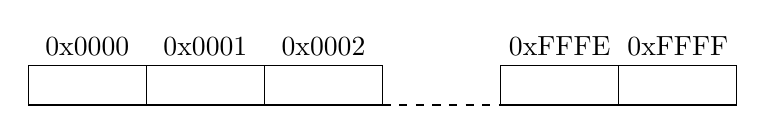
\begin{tikzpicture}[yscale=0.5, xscale=1.5]

    \draw (0,0) rectangle (1,1);
    \draw (1,0) rectangle (2,1);
    \draw (2,0) rectangle (3,1);
    \draw [dashed] (3,0) -- (4,0);
    \draw (4,0) rectangle (5,1);
    \draw (5,0) rectangle (6,1);
    \node  [above] at (0.5, 1) {0x0000};
    \node  [above] at (1.5, 1) {0x0001};
    \node  [above] at (2.5, 1) {0x0002};
    \node  [above] at (4.5, 1) {0xFFFE};
    \node  [above] at (5.5, 1) {0xFFFF};
\end{tikzpicture}
\caption{Bộ nhớ địa chỉ 16-bit} 
\end{figure}

Vậy mỗi ô nhớ sẽ có 2 thông số mà bạn cần quan tâm: địa chỉ (nó ở đâu, địa chỉ có thể là số 8-bit, 16-bit, 32-bit...), và giá trị được lưu (nó bao nhiêu, chỉ là số 8-bit (1 byte) thôi).

\begin{figure}[h!]
\centering
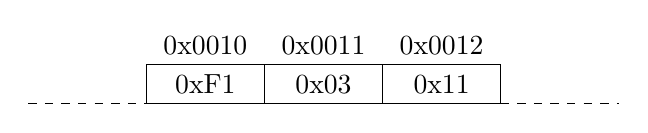
\begin{tikzpicture}[yscale=0.5, xscale=1.5]
    \draw [dashed] (0,0) -- (1,0);
    \draw (1,0) rectangle (2,1);
    \draw (2,0) rectangle (3,1);
    \draw (3,0) rectangle (4,1);
    \draw [dashed] (4,0) -- (5,0);
    
    \node  [above] at (1.5, 1) {0x0010};
    \node  [above] at (2.5, 1) {0x0011};
    \node  [above] at (3.5, 1) {0x0012};
    \node   at (1.5, 0.5) {0xF1};
    \node   at (2.5, 0.5) {0x03};
    \node   at (3.5, 0.5) {0x11};

\end{tikzpicture}
\caption{Dữ liệu trong bộ nhớ} %\label{fig: Dữ liệu trong bộ nhớ}
\end{figure}



Đoạn chương trình để xem địa chỉ trong DevC++:\*
\begin{lstlisting}
#include <stdio.h>
void main(){
    char a;
    printf("a address: 0x%08x\n", &a);
}
\end{lstlisting}


\section{Khai báo biến}

Các kiểu biến thông thường khi lập trình C là char, int, long, float, double. Nhưng trong lập trình nhúng, tài nguyên bộ nhớ hạn chế nên việc bạn biết các biến chiếm bao nhiêu ô nhớ là điều rất quan trọng. Thông thường, các biến được khai báo dưới dạng uint8\_t, int8\_t, uint16\_t, int16\_t... để sử dụng thì bạn cần  \#include <stdint.h>. Đoán xem mỗi kiểu sẽ chiếm bao nhiêu ô nhớ, và kiểu nào là kiểu có dấu, không đấu?

Một điểm đặc biệt là kiểu uint8\_t thường được dùng để đại diện cho một ô nhớ (8-bit). Ví dụ khi khai báo uint8\_t array[3], thì có thể hiểu là khai báo 3 phần tử mảng array có kiểu là uint8\_t, hoặc cũng có thể hiểu là yêu cầu bộ nhớ cấp 3 ô nhớ kề nhau. Các kiểu như byte hoặc char cũng có thể được dùng làm việc này nhưng mình vẫn thích sử dụng uint8\_t. Các khai báo các bộ đệm trong các giao tiếp như uart, i2c, spi... thường dùng kiểu biến này.

Thế nên hãy thường sử dụng các kiểu dữ liệu với bộ nhớ tường minh trên để kiểm soát bộ nhớ chặt chẽ hơn.\\
\section{Kiểu dữ liệu tự định nghĩa}

Ngôn ngữ C cung cấp cơ chế tự định nghĩa kiểu dữ liệu để việc truy xuất dữ liệu được thuận tiện.


Ví dụ mình có một cái cảm biến có thể đọc về nhiệt độ, độ ẩm và ánh sáng môi trường. Dữ liệu nhiệt độ từ  -20\textdegree{}C đến 100\textdegree{}C, độ ẩm từ 0\% đến 100\%, ánh sáng từ 0 lux đến 50.000 lux. Vậy mình khai báo dữ kiểu dữ liệu env\_t (environment type) như sau: 
\begin{lstlisting}
typedef struct{
    int8_t temp;
    uint8_t humi;
    uint16_t lux;
}env_t;
\end{lstlisting}

Dễ thấy là các kiểu biến bên trong đều chứa đủ khoảng giá trị cần thiết (nếu nhiệt độ vượt quá 127\textdegree{}C thì biến int8\_t không chứa được, phải chọn kiểu khác).

Thực chất kiểu dữ liệu là cách bạn tương tác với một vùng nhớ cho trước. Ví dụ khi khai báo một biến như \textit{env\_t env;} chẳng hạn, nó sẽ cung cấp cho bạn 4 ô nhớ liền nhau. Nếu bạn in địa chỉ của biến env ra nó sẽ hiển thị địa chỉ ô nhớ \textbf{đầu tiên} của dãy 4 ô nhớ đó. Và kiểu env\_t sẽ cho máy tính biết cách truy cập tới 4 ô nhớ đó như thế nào.

\begin{figure}[h!]
\centering
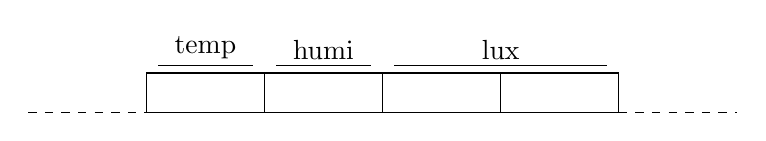
\begin{tikzpicture}[yscale=0.5, xscale=1.5]
    \draw [dashed] (0,0) -- (1,0);
    \draw (1,0) rectangle (2,1);
    \draw (2,0) rectangle (3,1);
    \draw (3,0) rectangle (4,1);
    \draw (4,0) rectangle (5,1);
    \draw [dashed] (5,0) -- (6,0);
    
    \draw (1.1, 1.2) -- (1.9, 1.2);
    \node [above] at (1.5, 1.1) {temp};
    
    \draw (2.1, 1.2) -- (2.9, 1.2);
    \node [above] at (2.5, 1.1) {humi};
    
    \draw (3.1, 1.2) -- (4.9, 1.2);
    \node [above] at (4, 1.1) {lux};
    
\end{tikzpicture}
\caption{Truy cập biến kiểu env\_t} %\label{fig: Dữ liệu trong bộ nhớ}
\end{figure}

Đoạn chương trình xem độ dài của kiểu dữ liệu:
\begin{lstlisting}
#include <stdio.h>
#include <stdint.h>

typedef struct{
int8_t temp;
uint8_t humi;
uint16_t lux;
}env_t;

void main(void) {
printf("Size of env_t: %d\n", sizeof(env_t));
}
\end{lstlisting}

Một điểm cần lưu ý là các máy tính thường có cơ chế làm tròn biên kiểu dữ liệu (data structure alignment). Nếu chúng ta khai báo như sau:

\begin{lstlisting}
typedef struct{
int8_t temp;
uint16_t lux;
uint8_t humi;
}env_t;
\end{lstlisting}
biến lux khai báo ở giữa, thì kiểu dữ liệu env\_t giờ đây có độ dài là 6 byte chứ không phải 4!!!.

Kiểu biến env\_t giờ có cấu trúc như sau:
\begin{figure}[h!]
\centering
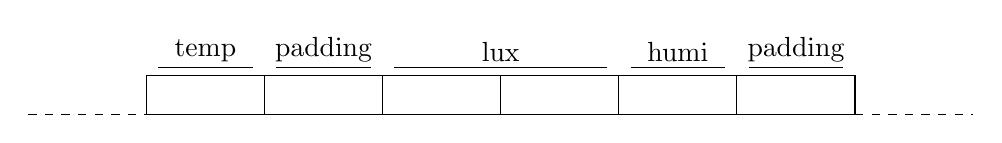
\begin{tikzpicture}[yscale=0.5, xscale=1.5]
    \draw [dashed] (0,0) -- (1,0);
    \draw (1,0) rectangle (2,1);
    \draw (2,0) rectangle (3,1);
    \draw (3,0) rectangle (4,1);
    \draw (4,0) rectangle (5,1);
    \draw (5,0) rectangle (6,1);
    \draw (6,0) rectangle (7,1);
    \draw [dashed] (7,0) -- (8,0);
    
    \draw (1.1, 1.2) -- (1.9, 1.2);
    \node [above] at (1.5, 1.1) {temp};
    
    \draw (2.1, 1.2) -- (2.9, 1.2);
    \node [above] at (2.5, 1.1) {padding};
    
    \draw (3.1, 1.2) -- (4.9, 1.2);
    \node [above] at (4, 1.1) {lux};
    
    \draw (5.1, 1.2) -- (5.9, 1.2);
    \node [above] at (5.5, 1.1) {humi};
    
    \draw (6.1, 1.2) -- (6.9, 1.2);
    \node [above] at (6.5, 1.1) {padding};
\end{tikzpicture}
\caption{Truy cập biến kiểu env\_t} 
\end{figure}

Hai ô nhớ tên padding được thêm vào để tăng hiệu suất việc đọc ghi dữ liệu trong máy tính hiện đại. Các bạn quan tâm thì có thể tìm hiểu thêm. Ta có thể tránh nó bằng cách khai báo như sau: trong DevC++ thì bạn khai báo \textit{\#pragma pack(1)} trước khi khai báo biến dữ liệu, còn trong nếu sử dụng KeilC cho chip STM32 hoặc kit Tiva thì khai báo kiểu:

\begin{lstlisting}
typedef __packed struct{
int8_t temp;
uint16_t lux;
uint8_t humi;
}env_t;
\end{lstlisting}
mỗi khi khai báo một kiểu biến nào đó. Trong Arduino thì mình không thấy nó có cơ chế này.


Ngoài ra còn một số kiểu enum và union mà các bạn hỏi giáo sư gu gồ hen.

\section{Con trỏ}

Có thể nói con trỏ là công cụ lợi hại nhất của C, bạn khó mà giỏi C nếu bỏ qua con trỏ được. Bản chất của con trỏ (chưa nói đến con trỏ hàm) là trỏ tới một vùng nhớ nào đó và tương tác với vùng nhớ đó. Chương trình ví dụ về con trỏ:
\begin{lstlisting}
#include <stdio.h>
#include <stdint.h>

int main(void) {
uint16_t a=0;
uint16_t *pa;
pa=&a;
printf("a addr: 0x%08x\n", &a);
printf("a addr: 0x%08x\n", pa);
}
\end{lstlisting}

hai lần printf sẽ cho ra kết quả như nhau vì đã gán địa chỉ của a cho pa.

Lưu ý là bạn không cần quan tâm địa chỉ thật của a (có dạng số hex như 0x0012) chỉ cần khai báo biến a, nó sẽ nằm đâu đó trong RAM (nếu RAM còn trống) và có phép lấy địa chỉ \&a.

Một con trỏ cần 2 thông tin sau để có thể hoạt động được: \textbf{địa chỉ} và \textbf{kiểu dữ liệu} nó sẽ trỏ tới. Như chương trình trên thì dòng số 6 sẽ cấp cho con trỏ kiểu dữ liệu, dòng số 7 cấp địa chỉ. 2 yếu tố trên giúp bạn có thể đi đến vùng nhớ mà bạn quan tâm sau đó có thể truy cập vùng nhớ đó theo cách bạn muốn.

Một lưu ý là ngôn ngữ C đồng nhất giữa mảng và con trỏ. Ví dụ mình khai báo mảng uint32\_t arr[4], thì \textit{arr} là địa chỉ của phần tử đầu tiên của mảng, hay arr=\&arr[0] (cùng 1 địa chỉ), *arr=arr[0] (cùng 1 giá trị). Giả sử arr là địa chỉ 0x0010 thì arr+1 sẽ là địa chỉ của arr[1] có địa chỉ là 0x0014 (không phải 0x0011 he, đo mỗi biến có 4 ô nhớ, kiểm tra lại bằng DevC++).
\section{Ví dụ về truyền nhận uart}


Để biết con trỏ nó lợi hại như thế nào thì các bạn hãy xem ví dụ về truyền nhận uart.

Các hàm truyền nhận dữ liệu uart thường có cấu trúc như sau:
\begin{lstlisting}
uart_transmit(uint8_t *data, uint16_t size);
uart_receive(uint8_t *data, uint16_t size);
\end{lstlisting}

Trong hàm uart\_transmit, tham số *data là ô nhớ đầu tiên trong chuỗi ô nhớ liên tiếp mà bạn muốn gửi đi. Còn trong hàm uart\_receive, tham số *data là ô nhớ đầu tiên của vùng nhớ mà bạn sẽ cất dữ liệu nhận được vào đấy (địa chỉ bộ đệm).
\subsection{Truyền uart}

Mình ví dụ chương trình sau: một MCU đọc cảm biến môi trường, lưu vào biến env (khai báo ở trên), rồi truyền qua đường uart về một MCU khác để xử lý.


Vậy giờ mình cần gửi một biến env (khi đã nhập dữ liệu cho biến này) đi thì cần làm thế nào để hàm truyền kia có thể truyền một kiểu env\_t đi trong khi hàm truyền nhận uart chỉ nhận vào là kiểu uint8\_t?

Cách giải quyết của mình là thế này, tạo một con trỏ kiểu uint8\_t và cấp cho nó địa chỉ của biến env.
\begin{lstlisting}
env_t env; //env.temp=10; env.humi=70, env.lux=1000;
uint8_t *pe;
pe=(uint8_t *)&env;
uart_transmit(pe, sizeof(env_t));
\end{lstlisting}

Câu lệnh dòng số 3, \textit{pe=(uint8\_t *)\&env} có 2 phần: đầu tiên là \&env, lấy địa chỉ của biến env tạo thành một con trỏ tạm thời kiểu env\_t, sau đó ép kiểu con trỏ (uint8\_t *) và gán cho pe. Vậy pe là một con trỏ kiểu uint8\_t và có địa chỉ của biến env, sau đó mình dùng hàm uart truyền đi 4 ô nhớ bắt đầu từ ô nhớ này. Mấy bạn chưa quen thì nên ngâm cứu kĩ chỗ này :)))

Khi sử dụng đến con trỏ, bạn cần có \textbf{tư duy ở ô nhớ} (chứ không phải kiểu dữ liệu) thì việc sử dụng con trỏ sẽ đơn giản hơn rất nhiều. Ví dụ như trong hàm truyền uart, với kiểu uint8\_t đại diện cho ô nhớ, và hai tham số *data và size, có ý nói là hãy đưa tôi địa chỉ ô nhớ đầu tiên và số lượng cần truyền, tôi sẽ truyền cái đống đó đi cho bạn.
\subsection{Nhận uart}

Phía nhận muốn nhận được dữ liệu thì trước tiên phải khai báo một bộ đệm, sau đó gọi hàm uart\_receive() trỏ tới bộ đệm này và chờ dữ liệu đến.
\begin{lstlisting}
#define MAX_BUFF 10
uint8_t uart_buffer[MAX_BUFF];
uart_receive(uart_buffer, sizeof(env_t));
\end{lstlisting}

Lưu ý là số lượng ô nhớ của bộ đệm phải lớn hớn hoặc bằng số lượng trong một lần truyền, nếu không chương trình sẽ lỗi. Câu lệnh số 1 để định nghĩa số lượng và để lên trên cùng của trang để sau này sửa lại số lượng cho phù hợp (cỡ như chương trình của bạn 1000 dòng mà nhét thẳng số 10 vô khai báo mảng luôn mai mốt tìm lại đuối).

Rồi, sau khi nhận được dữ liệu, việc của bạn là đọc dữ liệu và hiển thị lên màn hình lcd hoặc cất đâu đó. Ta tiến hành ép kiểu một lần nữa
\begin{lstlisting}
env_t *p_env;
p_env = (env_t *)uart_buffer;

\end{lstlisting}
để có được con trỏ kiểu env\_t và trỏ đến vùng nhớ ta vừa nhận được. Sau đó ta có thể sử dụng con trỏ này.
\begin{lstlisting}
printf("Temperature: %d\n", p_env->temp);
printf("Humidity: %d\n", p_env->humi);
printf("Lux: %d\n", p_env->lux);

\end{lstlisting}

Như vậy là cùng nhiêu đó ô nhớ nhưng \textbf{cách nhìn các ô nhớ đó} khác nhau với những kiểu dữ liệu khác nhau. Việc ép kiểu không làm thay đổi nội dung của ô nhớ vật lý (nó vẫn là cái đống 00 11 đó thôi), nhưng nó thay đổi cách bạn đọc nó.
\begin{figure}[h!]
\centering
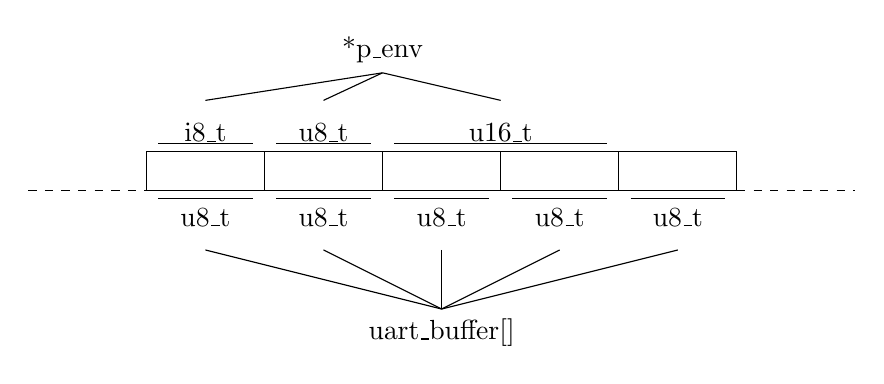
\begin{tikzpicture}[yscale=0.5, xscale=1.5]
    \draw [dashed] (0,0) -- (1,0);
    \draw (1,0) rectangle (2,1);
    \draw (2,0) rectangle (3,1);
    \draw (3,0) rectangle (4,1);
    \draw (4,0) rectangle (5,1);
    \draw (5,0) rectangle (6,1);
    \draw [dashed] (6,0) -- (7,0);
    
    \draw (1.1, 1.2) -- (1.9, 1.2);
    \node [above] at (1.5, 1) {i8\_t};
    \draw (1.5,2.3)--(3,3);		
    
    \draw (2.1, 1.2) -- (2.9, 1.2);
    \node [above] at (2.5, 1) {u8\_t};
    \draw (2.5,2.3)--(3,3);		
    
    \draw (3.1, 1.2) -- (4.9, 1.2);
    \node [above] at (4, 1) {u16\_t};
    \draw (4,2.3)--(3,3);	
    
    \node [above] at (3, 3) {*p\_env};
    
    \draw (1.1, -0.2) --(1.9,-0.2);
    \node [below] at (1.5, -0.2) {u8\_t};
    \draw (1.5, -1.5) -- (3.5,-3);

    \draw (2.1, -0.2) --(2.9,-0.2);
    \node [below] at (2.5, -0.2) {u8\_t};
    \draw (2.5, -1.5) -- (3.5,-3);

    \draw (3.1, -0.2) --(3.9,-0.2);
    \node [below] at (3.5, -0.2) {u8\_t};
    \draw (3.5, -1.5) -- (3.5,-3);

    \draw (4.1, -0.2) --(4.9,-0.2);
    \node [below] at (4.5, -0.2) {u8\_t};
    \draw (4.5, -1.5) -- (3.5,-3);

    \draw (5.1, -0.2) --(5.9,-0.2);
    \node [below] at (5.5, -0.2) {u8\_t};
    \draw (5.5, -1.5) -- (3.5,-3);
    
    \node [below] at (3.5, -3) {uart\_buffer[]};
    
\end{tikzpicture}
\caption{Buffer v.s env\_t.}
\end{figure}

Rồi đến đây các bạn có thể cảm nhận được sức mạnh của con trỏ rồi, bạn có thể \textbf{chạm} đến bất cứ vùng nhớ nào và truy xuất theo \textbf{kiểu} mà bạn muốn. Thiệc là dễ quá chừng :))

Có một cách hiểu khác thế này, mỗi khi khai báo một con trỏ với một kiểu dữ liệu nào đấy, bạn đang khai báo một cái \textbf{mặt nạ}, hay một \textbf{cách}, một \textbf{phương thức} để khai thác dữ liệu.
\begin{figure}[h!]
\centering
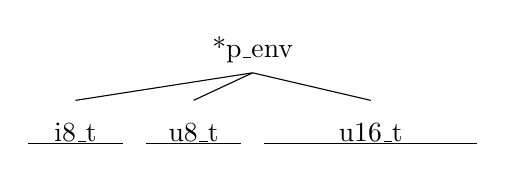
\begin{tikzpicture}[yscale=0.5, xscale=1.5]

    \draw (1.1, 1.2) -- (1.9, 1.2);
    \node [above] at (1.5, 1) {i8\_t};
    \draw (1.5,2.3)--(3,3);		
    
    \draw (2.1, 1.2) -- (2.9, 1.2);
    \node [above] at (2.5, 1) {u8\_t};
    \draw (2.5,2.3)--(3,3);		
    
    \draw (3.1, 1.2) -- (4.9, 1.2);
    \node [above] at (4, 1) {u16\_t};
    \draw (4,2.3)--(3,3);	
    
    \node [above] at (3, 3) {*p\_env};

\end{tikzpicture}
\caption{The mask}
\end{figure}

Bạn chưa thể đọc được dữ liệu nào cả vì mới chỉ khai báo cái cách truy cập dữ liệu thôi. Còn khi cấp địa chỉ cho con trỏ thì bạn đang ráp cái mặt nạ đó vào một hàng ô nhớ thực và sau có thể truy cập các ô nhớ đó theo cách này (hình 2.7).

\begin{figure}[h!]
\centering
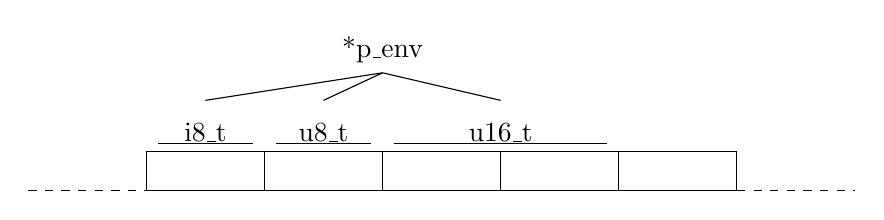
\begin{tikzpicture}[yscale=0.5, xscale=1.5]
    \draw [dashed] (0,0) -- (1,0);
    \draw (1,0) rectangle (2,1);
    \draw (2,0) rectangle (3,1);
    \draw (3,0) rectangle (4,1);
    \draw (4,0) rectangle (5,1);
    \draw (5,0) rectangle (6,1);
    \draw [dashed] (6,0) -- (7,0);
    
    \draw (1.1, 1.2) -- (1.9, 1.2);
    \node [above] at (1.5, 1) {i8\_t};
    \draw (1.5,2.3)--(3,3);		
    
    \draw (2.1, 1.2) -- (2.9, 1.2);
    \node [above] at (2.5, 1) {u8\_t};
    \draw (2.5,2.3)--(3,3);		
    
    \draw (3.1, 1.2) -- (4.9, 1.2);
    \node [above] at (4, 1) {u16\_t};
    \draw (4,2.3)--(3,3);	
    
    \node [above] at (3, 3) {*p\_env};
    
\end{tikzpicture}
\caption{The mask and the data.}
\end{figure}
\newpage

Lưu ý: bộ đêm là nơi dữ liệu đến và đi liên tục, nó là bến đỗ chứ không phải là chỗ chứa dữ liệu. Dữ liệu mới ập đến có thể ghi đè lên dữ liệu cũ. Nên cất vào đâu đấy rồi hãy xử lý gì đó tiếp theo
\begin{lstlisting}
env_t *p_env;
p_env = (env_t *)uart_buffer;
env_t recv_env=*p_env;
printf("Temperature: %d\n",  recv_env.temp);
printf("Humidity: %d\n",  recv_env.humi);
printf("Lux: %d\n",  recv_env.lux);
\end{lstlisting}
và việc ép kiểu này chỉ đúng nếu hai bên gửi và nhận có cùng cơ chế bộ nhớ hoặc big-endian hoặc little-endian thôi. Nếu khác kiểu thì không sử dụng được.
\section{Debug}

Khi viết một chương trình thì nhất thiết phải có công cụ để theo dõi coi code của bạn nó đang làm cái gì ở trỏng. Nếu ở lập trình C thuần túy bằng cái IDE như DevC++ hoặc Visual Studio thì bạn chỉ cần gọi hàm printf ra và in cái gì trong đó bạn muốn. Còn trong lập trình nhúng thì con MCU của bạn nó chạy chứ không phải CPU của máy tính. Muốn MCU in ra được những dòng chữ lên màn hình desktop thì cần theo quy trình sau: MCU truyền qua uart, qua một module chuyển uart-usb đã cắm vào máy tính, một chương trình đọc cổng COM trên máy tính và hiển thị chuỗi kí tự nhận được.

Trên board Arduino có sẵn bộ chuyển usb-uart rồi, thường là cổng uart 0 (Serial 0). Code để demo mình đã để sẵn trên \textit{\url{https://github.com/congkeodhbk/Lap_trinh_nhung}}. 

Có 2 board, một cái nạp chương trình transmit và một cái nạp receive. Chương trình transmit liên tục gửi biến về. Còn receive thì đọc và hiển thị kết quả. Tuy nhiên bên receive nó hơi phức tạp xíu. Giả sử mình nhận mà không biết thằng gửi sẽ gửi bao nhiêu byte thì sao? Vậy mình sẽ sử dụng cách đại khái là khi nó đang nhận mà không thấy dữ liệu đến nữa trong vòng 20 mili giây thì nó hiểu là đã nhận xong. Các bạn đọc code rồi mò coi cắm chân cẳng thế nào để cái đứa nói chuyện được với nhau. Và xa hơn bạn thử lấy môt cái chip khác, như stm32f4 chẳng hạn, viết chương trình tương tự code transmit và gửi cho Arduino receive nhận xem nó có chạy không (hai tên đó một đứa 3v3 với một đứa 5v, phải có mạch chuyển mức logic, không cắm thẳng vào, sẽ xịt khói). Và xa tới đầu hẻm nữa thì viết tất cả mọi thứ lên chip khác, cả thư viện debug của mình.

Trong thư viện trên mới chỉ có hàm debug() tương đương với printf() trong C, còn nhiều cách debug xịn hơn, như làm thế nào sử dụng lệnh tương tự scanf trong C lên board Arduino, bạn nhập lệnh trên màn hình console của máy tính và chuyển xuống Arduino, tùy mỗi lệnh bạn nhập mà nó chạy những kịch bản khác nhau.
